%% This is file `elsarticle-template-1-num.tex',
%%
%% Copyright 2009 Elsevier Ltd
%%
%% This file is part of the 'Elsarticle Bundle'.
%% ---------------------------------------------
%%
%% It may be distributed under the conditions of the LaTeX Project Public
%% License, either version 1.2 of this license or (at your option) any
%% later version.  The latest version of this license is in
%%    http://www.latex-project.org/lppl.txt
%% and version 1.2 or later is part of all distributions of LaTeX
%% version 1999/12/01 or later.
%%
%% The list of all files belonging to the 'Elsarticle Bundle' is
%% given in the file `manifest.txt'.
%%
%% Template article for Elsevier's document class `elsarticle'
%% with numbered style bibliographic references
%%
%% $Id: elsarticle-template-1-num.tex 149 2009-10-08 05:01:15Z rishi $
%% $URL: http://lenova.river-valley.com/svn/elsbst/trunk/elsarticle-template-1-num.tex $
%%
\documentclass[preprint,12pt]{elsarticle}

%% Use the option review to obtain double line spacing
%% \documentclass[preprint,review,12pt]{elsarticle}

%% Use the options 1p,twocolumn; 3p; 3p,twocolumn; 5p; or 5p,twocolumn
%% for a journal layout:
%% \documentclass[final,1p,times]{elsarticle}
%% \documentclass[final,1p,times,twocolumn]{elsarticle}
%% \documentclass[final,3p,times]{elsarticle}
%% \documentclass[final,3p,times,twocolumn]{elsarticle}
%% \documentclass[final,5p,times]{elsarticle}
%% \documentclass[final,5p,times,twocolumn]{elsarticle}

\usepackage{cite}

%% if you use PostScript figures in your article
%% use the graphics package for simple commands
%% \usepackage{graphics}
%% or use the graphicx package for more complicated commands
\usepackage{graphicx}
%% or use the epsfig package if you prefer to use the old commands
%% \usepackage{epsfig}
\usepackage{epstopdf}

%% The amssymb package provides various useful mathematical symbols
\usepackage{amssymb, amsmath}
%% The amsthm package provides extended theorem environments
%% \usepackage{amsthm}

%% The lineno packages adds line numbers. Start line numbering with
%% \begin{linenumbers}, end it with \end{linenumbers}. Or switch it on
%% for the whole article with \linenumbers after \end{frontmatter}.
\usepackage{lineno}

%% natbib.sty is loaded by default. However, natbib options can be
%% provided with \biboptions{...} command. Following options are
%% valid:

%%   round  -  round parentheses are used (default)
%%   square -  square brackets are used   [option]
%%   curly  -  curly braces are used      {option}
%%   angle  -  angle brackets are used    <option>
%%   semicolon  -  multiple citations separated by semi-colon
%%   colon  - same as semicolon, an earlier confusion
%%   comma  -  separated by comma
%%   numbers-  selects numerical citations
%%   super  -  numerical citations as superscripts
%%   sort   -  sorts multiple citations according to order in ref. list
%%   sort&compress   -  like sort, but also compresses numerical citations
%%   compress - compresses without sorting
%%
%% \biboptions{comma,round}

% \biboptions{}

\begin{document}

\begin{frontmatter}

%% Title, authors and addresses

%% use the tnoteref command within \title for footnotes;
%% use the tnotetext command for the associated footnote;
%% use the fnref command within \author or \address for footnotes;
%% use the fntext command for the associated footnote;
%% use the corref command within \author for corresponding author footnotes;
%% use the cortext command for the associated footnote;
%% use the ead command for the email address,
%% and the form \ead[url] for the home page:
%%
%% \title{Title\tnoteref{label1}}
%% \tnotetext[label1]{}
%% \author{Name\corref{cor1}\fnref{label2}}
%% \ead{email address}
%% \ead[url]{home page}
%% \fntext[label2]{}
%% \cortext[cor1]{}
%% \address{Address\fnref{label3}}
%% \fntext[label3]{}

\title{Linear Prediction of Speech}

%% use optional labels to link authors explicitly to addresses:
%% \author[label1,label2]{<author name>}
%% \address[label1]{<address>}
%% \address[label2]{<address>}

\author{Yu Cang}
\address{Shanghai Jiao Tong University, China}

\begin{abstract}
%% Text of abstract
A model was established for predicting a speech linearly. Two strategies are developed to determine the coefficients. One is windowing the signal and the Topelitz equations are solved iteratively. The other is windowing the error and the Cholesky decomposition is applied. Both the two strategies are compared with a sample speech finally.
\end{abstract}

\begin{keyword}
Speech Prediction \sep Correlation \sep Covariance \sep Cholesky \sep Topelitz
%% keywords here, in the form: keyword \sep keyword

%% MSC codes here, in the form: \MSC code \sep code
%% or \MSC[2008] code \sep code (2000 is the default)

\end{keyword}

\end{frontmatter}

%%
%% Start line numbering here if you want
%%
%\linenumbers

%% main text
\section{Basic Equations}
\label{S:1}
In a simplified situation, a speech can be linearly predicted from the previous $p$ samples as
\begin{equation}
	\hat{x}(n) =  \sum_{i=1}^{p} a_i x(n-i)
\end{equation}
where $a_i$ are the linear prediction coefficients. Then the error between the signal $x(n)$ and the predicted value $\hat{x}(n)$ is given as
\begin{equation}
	e(n) = x(n) - \hat{x}(n) = -\sum_{i=0}^{p}a_i x(n-i)
\end{equation}
where $a_0 = -1$. The minimum mean square error(MMSE) is adopted as the principle to determine these coefficients $a_i$.

The square error of the prediction is defined as
\begin{equation}
	E = \sum_{n}e^2(n) = \sum_{n}[x(n) - \sum_{i=1}^{p}a_i x(n-i)]^2
\end{equation}
To minimize $E$, each coefficient $a_i\ (i = 1, 2, ..., p)$ is determined as
\begin{equation}
	\frac{\partial E}{\partial a_i} = 0
\end{equation}
Which is equivalent to
\begin{equation}\label{coef_eqn}
	\sum_{j=1}^{p}a_j \sum_{n}x(n-j)x(n-i) = \sum_{n}x(n)x(n-i)
\end{equation}
where $i= 1, 2, ..., p$.

Denote $\phi(i,j)$ as
\begin{equation}\label{phi_def}
	\phi(i, j) = \sum_{n}x(n-i)x(n-j) 
\end{equation}
it's clear that $\phi(i,j) = \phi(j, i)$, and (\ref{coef_eqn}) can be written as
\begin{equation}
	\sum_{j=1}^{p} \phi(j, i)a_j = \phi(0, i)
\end{equation}
where $i= 1, 2, ..., p$.

Hence, it is left to determine $\phi(j, i)$ and then $a_j$ can be resolved. However, there're different ways to determine the bounds of $n$ when calculating $\phi(j, i)$, which led to different strategies of linear prediction.

\section{The Autocorrelation Method}\label{S:2}
The autocorrelation method aims to minimize the error over the whole timespan, and it's assumed that $x(n)$ is 0 when $n \notin [0,N-1]$. Thus, $x(n)$ is windowed with finite length, and the autocorrelation function of $x(n)$ is defined as
\begin{equation}
	r(j) = \sum_{n=-\infty}^{+\infty} x(n)x(n-j) \ \ (j \in [1, p])
\end{equation}
It can be concluded that, from (\ref{phi_def}), $r(|j-i|) = \phi(j, i)$. Thus, (\ref{coef_eqn}) can be expressed as
\begin{equation}
	\begin{bmatrix}
		r(0) & r(1) & r(2) & ... & r(p-1) \\ 
		r(1) & r(0) & r(1) & ... & r(p-2) \\
		r(2) & r(1) & r(0) & ... & r(p-3) \\
		\vdots & \vdots & \vdots & \ddots & \vdots \\
		r(p-1) & r(p-2) & r(p-3) & ... & r(0)
	\end{bmatrix}
	\begin{bmatrix}
	a_1 \\ a_2 \\ a_3 \\ \vdots \\ a_p
	\end{bmatrix}
	=
	\begin{bmatrix}
		r(1) \\ r(2) \\ r(3) \\ \vdots \\ r(p)
	\end{bmatrix}
\end{equation}
It can be observed that the coefficient matrix is the so called Toeplitz matrix, where elements are symmetry and  each descending diagonal from left to right is constant.

Suppose $a_i^{(k)} \ (i=1, 2, ... ,k)$ is the solution for $k-th$ iteration for $p=k$, which implies
\begin{equation}
	\begin{bmatrix}
		r(0) & r(1) & r(2) & ... & r(k-1) \\ 
		r(1) & r(0) & r(1) & ... & r(k-2) \\
		r(2) & r(1) & r(0) & ... & r(k-3) \\
		\vdots & \vdots & \vdots & \ddots & \vdots \\
		r(k-1) & r(k-2) & r(k-3) & ... & r(0)
	\end{bmatrix}
	\begin{bmatrix}
		a_1^{(k)} \\ a_2^{(k)} \\ a_3^{(k)} \\ \vdots \\ a_k^{(k)}
	\end{bmatrix}
	=
	\begin{bmatrix}
		r(1) \\ r(2) \\ r(3) \\ \vdots \\ r(k)
	\end{bmatrix}
\end{equation}
Thus, when $p=k+1$, two equation sets can be constructed as
\begin{equation}
	\begin{bmatrix}
		r(0) & r(1) & ... & r(k)\\ 
		r(1) & r(0) & ... & r(k-1)\\
		r(2) & r(1) & ... & r(k-2)\\
		\vdots & \vdots & \ddots & \vdots \\
		r(k-1) & r(k-2) & ... & r(1)\\
		r(k) & r(k-1) & ... & r(0)\\
	\end{bmatrix}
	\begin{bmatrix}
		a_1^{(k)} \\ a_2^{(k)} \\ a_3^{(k)} \\ \vdots \\ a_k^{(k)} \\ -\lambda
	\end{bmatrix}
	=
	\begin{bmatrix}
		r(1) - \lambda r(k) \\
		r(2) - \lambda r(k-1) \\
		r(3) - \lambda r(k-2) \\
		\vdots \\
		r(k) - \lambda r(1) \\
		\sum_{i=1}^{k}a_i^{(k)} r(k+1-i)-\lambda r(0)
	\end{bmatrix}
\end{equation}
and
\begin{equation}
	\begin{bmatrix}
		r(0) & r(1) & ... & r(k)\\ 
		r(1) & r(0) & ... & r(k-1)\\
		r(2) & r(1) & ... & r(k-2)\\
		\vdots & \vdots & \ddots & \vdots \\
		r(k-1) & r(k-2) & ... & r(1)\\
		r(k) & r(k-1) & ... & r(0)\\
	\end{bmatrix}
	\begin{bmatrix}
		\lambda a_k^{(k)} \\
		\lambda a_{k-1}^{(k)} \\
		\lambda a_{k-2}^{(k)} \\
		\vdots \\
		\lambda a_1^{(k)} \\
		0
	\end{bmatrix}
	=
	\begin{bmatrix}
		\lambda r(k) \\
		\lambda r(k-1) \\
		\lambda r(k-2) \\
		\vdots \\
		\lambda r(1) \\
		\lambda\sum_{i=1}^{k}a_i^{(k)} r(i)
	\end{bmatrix}
\end{equation}
Let $\lambda$ satisfy
\begin{equation}
	\sum_{i=1}^{k}a_i^{(k)} r(k+1-i)-\lambda r(0) + \lambda\sum_{i=1}^{k}a_i^{(k)} r(i) = r(k+1)
\end{equation}
namely
\begin{equation}
	\lambda = \frac{r(k+1) - \sum_{i=1}^{k}a_i^{(k)} r(k+1-i)}{\sum_{i=0}^{k}a_i^{(k)}r(i)}
\end{equation}
where $a_0^{(k)} = -1$. Then $a_i^{(k+1)}$ can be given as
\begin{equation}
	\{a_i^{(k+1)}\} = 
	\begin{bmatrix}
		a_1^{(k)} + \lambda a_k^{(k)} & a_2^{(k)} + \lambda a_{k-1}^{(k)} & ... & a_k^{(k)} + \lambda a_1^{(k)} & -\lambda  
	\end{bmatrix}^T
\end{equation}
And it can be easily verified that the recursion formula is also valid when $k=1,2$, thus this solution is justified by induction. 

Further, this is the so-called Levinson-Durbin algorithm, with time complexity $O(n^2)$, and it is much faster than solving it directly where time complexity is $O(n^3)$.

\section{The Covariance Method}
In constrast to the previous method, the covariance method doesn't windowed the signal. Instead, the amount of points used to calculate the error is fixed. And it aims to minimize the error.

Suppose the amount of points to calculate $r(j)$ is $N$, then by definition
\begin{equation}
	r(j) = \sum_{n=0}^{N-1}x(n)x(n-j) \ \ (j = 0, 1, ... , p)
\end{equation}
Thus, $N+p$ samples are needed for calculating all $r(j)$. And $r(j-i)$ can be expressed as 
\begin{equation}
	r(j-i) = \sum_{n=0}^{N-1} x(n-j)x(n-i) \triangleq c(j, i) \ \ (j = 0, 1, ... , p) 
\end{equation}
Thus, the prediction equation (\ref{coef_eqn}) can be written as
\begin{equation}
	\begin{bmatrix}
		c(1, 1) & c(1, 2) & ... & c(1, p)\\
		c(2, 1) & c(2, 2) & ... & c(2, p)\\
		\vdots  & \vdots  & \ddots & \vdots\\
		c(p, 1) & c(p, 2) & ... & c(p, p)\\
	\end{bmatrix}
	\begin{bmatrix}
		a_1 \\ a_2 \\ \vdots \\ a_p
	\end{bmatrix}
	=
	\begin{bmatrix}
		c(1, 0) \\ c(2, 0) \\ \vdots \\ c(p, 0)
	\end{bmatrix}
\end{equation}
Since $c(i, j) \neq c(i+k, j+k)$, the coefficient matrix above is no longer the Toeplitz matrix, and different scheme should be employed to solve this linear system.

It's clear that $c(i, j) = c(j, i)$, so it can be solved using the Cholesky decomposition. And the coefficient matrix can be decomposed as
\begin{equation}
	C = L L^T
\end{equation}
where $L$ is a lower triangle matrix. Onece $L$ is obtained, targeting $a_i$ can be easily calculated by
\begin{equation}
	\begin{aligned}
		y & = linsolve(L, b)\\
		{a_i} & = linsolve(L^T, y)
	\end{aligned}
\end{equation}

\section{Numerical Experiment}
A segment of audio is taken as the original signal, where $len = 120$ samples are included. 
\subsection{Comparison between the autocorrelation and covariance}
Numerical experiments indicates that the covariance method performs better than the autocorrelation method when $p$ is fixed($p=6$).

The autocorrelation method is examined in Fig(\ref{fig:performance_auto}). It can be seen from the left figure that the predicted signals fit the original signals well, only with slightly difference. The error between is much more apparent at peak area. Details of performance is given in the right figure.

\begin{figure}[!htbp]\centering	
	\begin{minipage}{6.5cm}
		\centering
		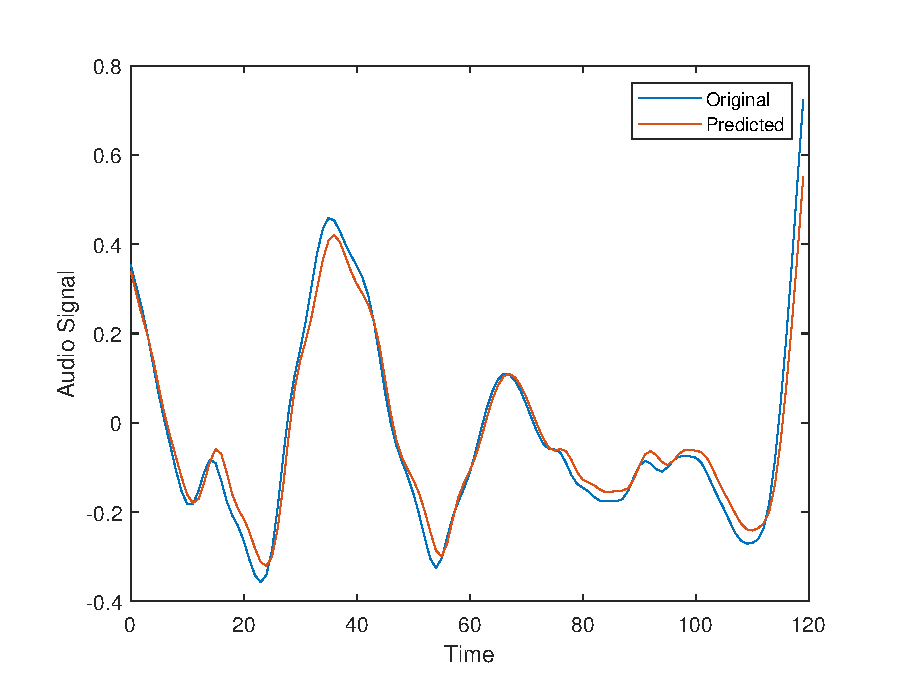
\includegraphics[height=6cm,width=7cm]{../pic/autocorrelation_120_6.eps}
	\end{minipage}
	\begin{minipage}{6.5cm}
		\centering
		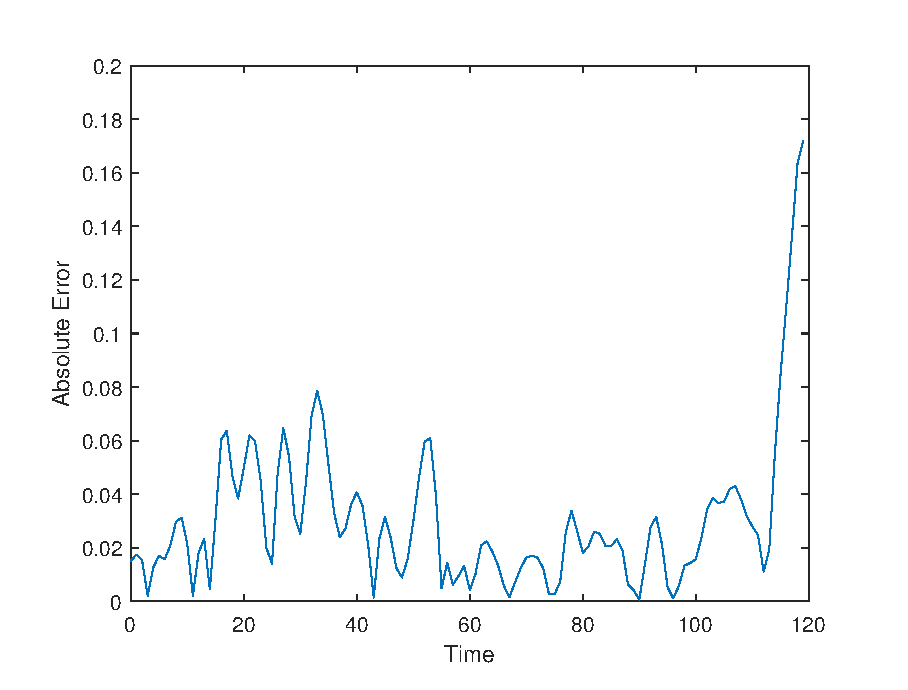
\includegraphics[height=6cm,width=7cm]{../pic/autocorrelation_err_120_6.eps}
	\end{minipage}
	\caption{Performance of the Autocorrelation Method}\label{fig:performance_auto}
\end{figure}

The covariance method is investigated in Fig(\ref{fig:performance_cov}). It can be seen from the left figure that the predicted signals meet the original signals very well and the error between is significantly eliminated compared to the autocorrelation method. It can be seen from the right figure that the error is lower by an order of magnitude.

\begin{figure}[!htbp]\centering	
	\begin{minipage}{6.5cm}
		\centering
		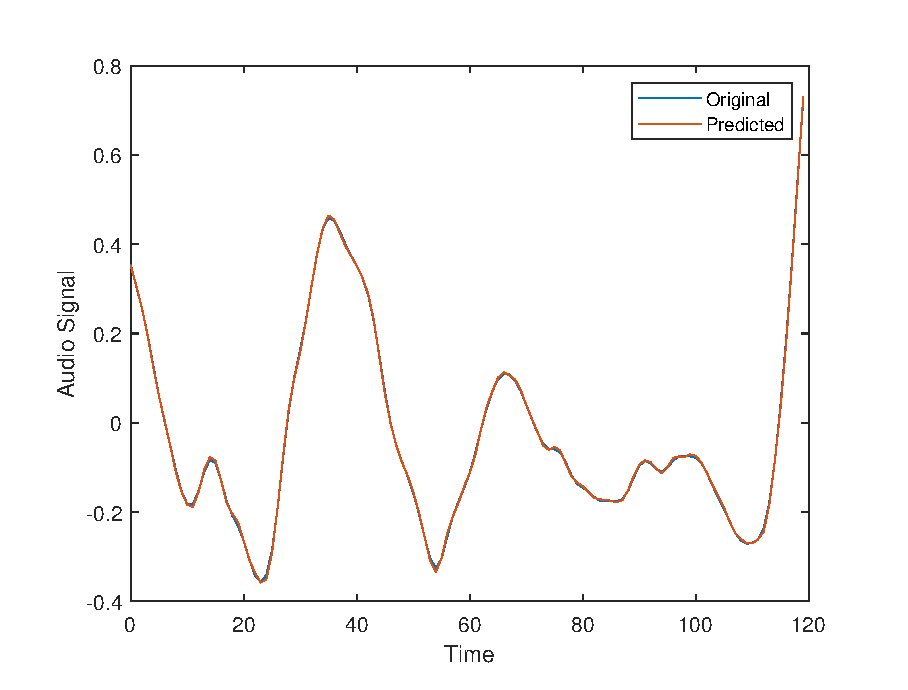
\includegraphics[height=6cm,width=7cm]{../pic/covariance_120_6.eps}
	\end{minipage}
	\begin{minipage}{6.5cm}
		\centering
		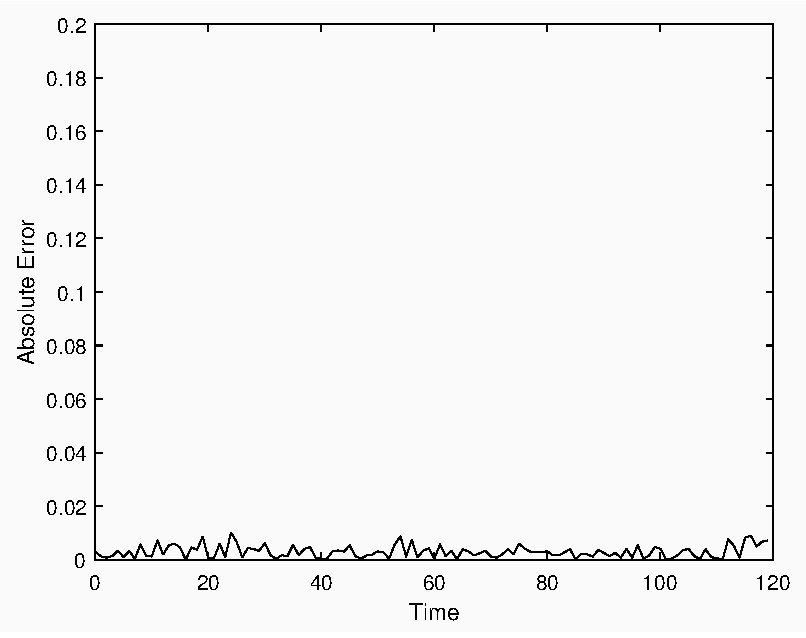
\includegraphics[height=6cm,width=7cm]{../pic/covariance_err_120_6.eps}
	\end{minipage}
	\caption{Performance of the Covariance Method}\label{fig:performance_cov}
\end{figure}

The difference can be explained as the bounds of $n$ are different. There're $p$ more points used in the covariance method when calculating the linear prediction coefficients, and hence, it's more likely that the covariance method out-performs the autocorrelation method.

\subsection{Relation between the error and $p$}
Here, the covariance method is choosen for further investigating the relation between the error and the prediction order $p$. 

Again, the total number of samples is fixed($len = 120$). The error vector $e$ is measured with $\lVert e \rVert_2$. $p$ is equidistantly choosen ranging from $2$ to $50$. Plot indicating the relation between the order of error and $p$ is given as below.

\begin{figure}[!h]
	\centering
	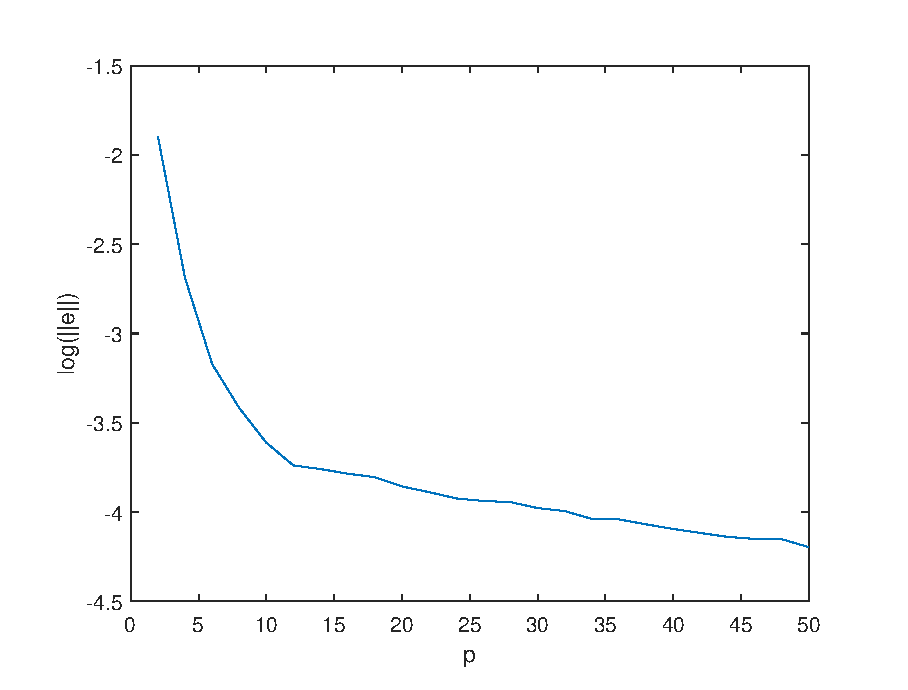
\includegraphics[height=5.5cm,width=9cm]{../pic/err_vs_p.eps}
\end{figure}

It can be seen from the plot that the error is reduced immediately when $p$ is increased from $5$ to $15$, but the error decreases slowly when $p$ continues to grow.

\section{Conclusion}
Two different methods were introduced to calculate the linear prediction coefficients. Numerical experiments were carried out to compare the performence of these two methods, and the results show that the covariance method
does better than the correlation method. Possible reasons were suggested and a further study on the relation between the error and $p$ indicates that the error decreases intensively at the begining but tends to be converged later on.

%% The Appendices part is started with the command \appendix;
%% appendix sections are then done as normal sections
%% \appendix

%% \section{}
%% \label{}

\bibliographystyle{plain}
\bibliography{article.bib}

\end{document}
